% !TEX root = ../main.tex

\section{Introductory Remarks}

Blockchain projects understand that even the best technical ideas and code can only achieve so much without user adoption of the platform. Projects struggle to reach users, who generally operate pseudonymously, and users do not always browse for new blockchain projects---there is no high profile `DApp store.'  One approach for introducing users to a new blockchain (including independent chains, sidechains, and layer 2 solutions) is showcasing its features and partners through gamification. A set of \textit{quests} or \textit{tasks} or \textit{boosts} are created that offer a \textit{bounty} or \textit{reward} to users for performing a specific action on the blockchain, such as transferring a token or using a specific DeFi service. The reward could be a collectable badge (often as an NFT), points on a leaderboard (often referred to as XP, inspired by games like Fortnite and platforms like Duolingo), or an airdrop of tokens with some monetary value. Most projects favour the term `quests' over `tasks' to avoid associations with employment. The term quest highlights the user's journey toward achievement and mastery, creating a more legally favourable framing rooted in gamification. Despite the aspirational tone, these actions remain structured and transactional, serving both users’ reward-driven motivations and projects’ growth and engagement objectives.

A few examples of quest initiatives include Arbitrum's Odyssey 2.0, Avalanche's Coachella Quests, Base's Builder Quests, Binance's BSC GameFi Quest and Polygon's Wallet Suite Quest. Platforms like Galxe, Layer3, Boost, DeBank, and Zealy have emerged as centralized hubs offering users a variety of quests from multiple projects and have adopted the description: the loyalty layer. 

In this measurements paper, we study one quest system over time to understand how the completion-rate of quests are influenced by factors such as difficulty, cost, reward amount, and reward type (monetary or non-monetary value). From our data, we are not able to directly classify users between humans and bots, however we do offer some insights and discussion points about the influence of automated task-completion. To inform this discussion, we identify key stakeholders involved (such as the blockchain, services on the blockchain, investors, activity monitoring services, users, and bots) and analyze their preferences and incentives. We maintain a neutral position on whether quests are useful or not---we study them because they are commonly used (perhaps poised for broader adoption) and we failed to find another detailed study on the parameters that impact task completion.

% = = = = = = = = = = = = = = = = = = = = = = = = = = = = = = = = = = = = = = = = = =

\subsection{Research Questions.} 
Our paper sheds light on the following research questions (RQs):

\begin{itemize}
\item \textbf{RQ1:} How does the reward amount impact completion?
\item \textbf{RQ2:} How does task difficulty impact completion?
\item \textbf{RQ3:} How does cost to the user impact completion?
\item \textbf{RQ4:} How does enforcing a minimum threshold of value held by the account impact completion?
\item \textbf{RQ5:} How does offering tokens of monetary value impact completion?
\item \textbf{RQ6:} To what extent can the design of the quest help distinguish regular users from automated bots and farming?
\end{itemize}

% = = = = = = = = = = = = = = = = = = = = = = = = = = = = = = = = = = = = = = = = = =

\subsection{Related Work}

Recent papers have studied airdrops of new tokens~\cite{FB19,MYL24,YL24}. Airdrops studied in this literature are large-scale events where a large quantity (majority to totality) of tokens are distributed to users for the first time. This literature finds a positive impact of airdrops on token value, that retaining user engagement after an airdrop is difficult, and evidence of artificial engagement to `farm' airdropped tokens. If a quest system predates an airdrop, quest completion can be a factor in determining airdrop recipients. 

Our research questions are influenced by a persuasion model called the Fogg Behaviour Model~\cite{Fogg09} which suggests certain deterrents to engagement: time, money, physical effort, brain cycles, social deviance, and non-routine. We examine the influence of quest difficultly (time, brain cycles, and non-routine) and cost (money) on completion, assuming most quests have similar levels of physical effort (minimal) and social deviance (legal or unregulated in most jurisdictions). 

% = = = = = = = = = = = = = = = = = = = = = = = = = = = = = = = = = = = = = = = = = =

\subsection{Dataset and Overview}

For our paper, we study a quest system built and maintained by a company offering a new blockchain. The quests themselves were co-designed with various services (DApps) running on the blockchain. All of our measurements are replicable from the public website and blockchain data. Our research analyzes data spanning the entirety of 2024. New quests are offered for an epoch, which was initially a one day period and transitioned (at epoch 10) to one week. Our data is organized by epoch 5 (no data was collected for epoch 1--4) to epoch 42. Over this period, 43 unique quests were offered. Some quests were offered in multiple epochs and could be completed multiple times. 1.2M unique addresses completed at least one quest.  Across the period, 80M quests were completed.

\begin{figure}[t]
    \centering
    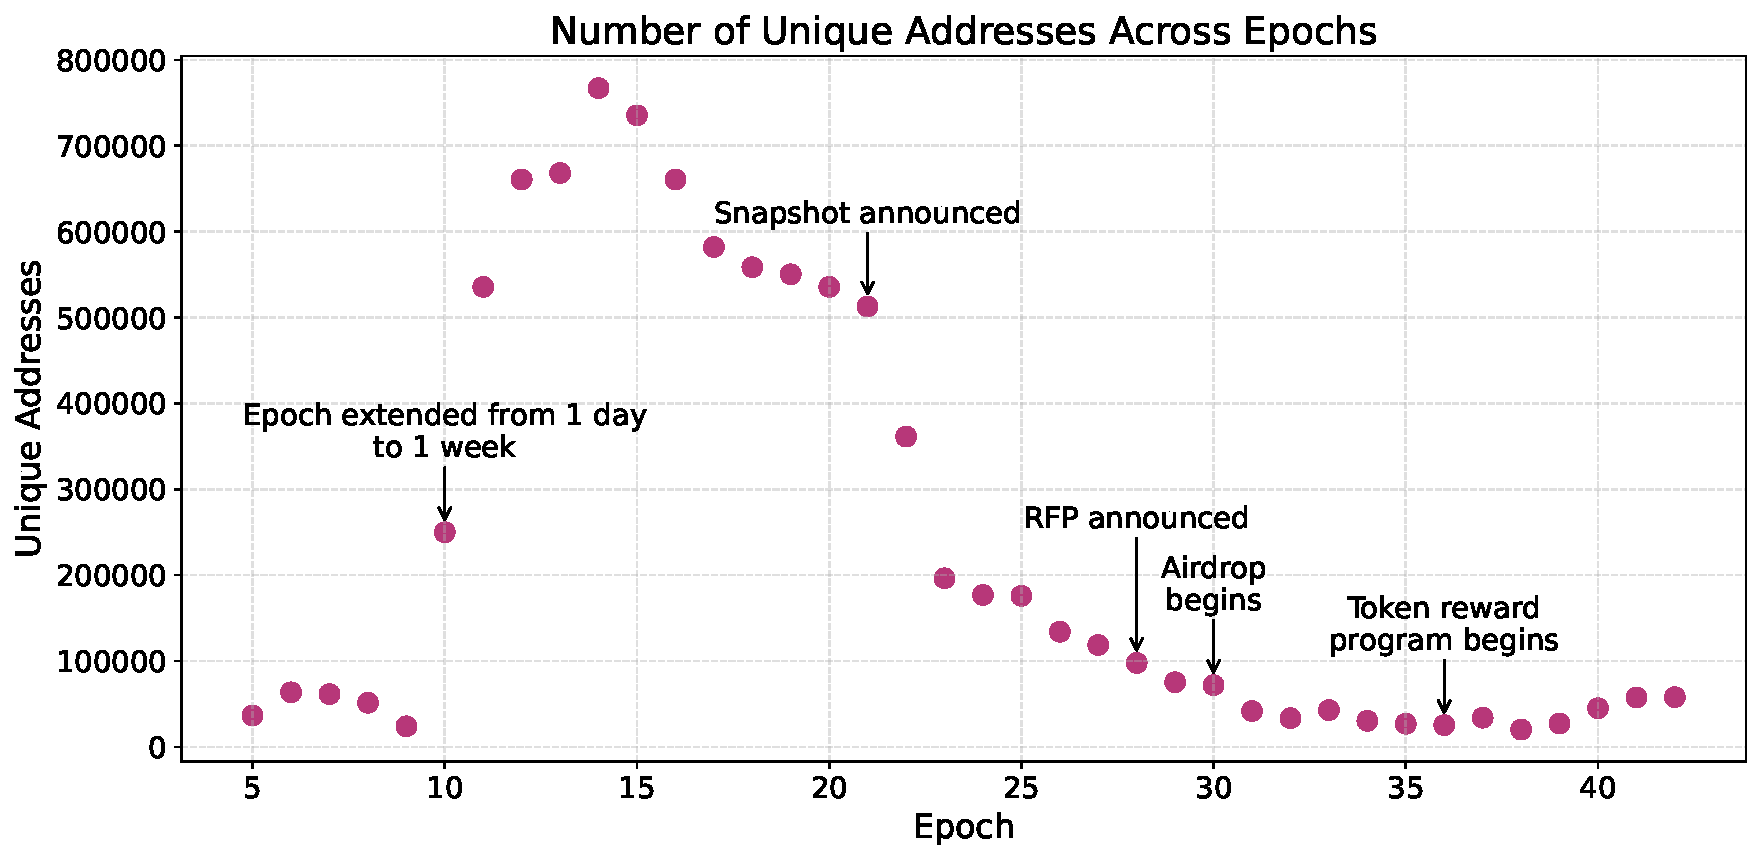
\includegraphics[width=0.8\textwidth]{figures/events.pdf}
    \caption{Total completions of all quests offered in each epoch. Overlay of public announcements that may impact user participation.}
    \label{fig:events}
\end{figure}

As seen in  Figure~\ref{fig:events}, overall participation seems to be influenced by various public announcements. When a blockchain does not offer a token but does offer quests, speculative users might assume that an airdrop of tokens is on the blockchain's future roadmap and quest completion points might factor into who receive airdropped tokens. At epoch 21, the project announces an airdrop and that a snapshot of user activity had been captured as a basis of for the airdrop. Since the snapshot is taken, it is too late to complete quests for the purposes of gaining in airdropped tokens (unless if you speculate that the project will do a second snapshot or a second airdrop). Participation dropped 29.5\% immediately after the snapshot announcement. By epoch 23, a further 45.7\% drop occurred, totalling a 61.7\% decline over two weeks. At epoch 28, a request for proposals (RFP) was announced to ask ecosystem apps and partners to submit how they want to do airdrop allocation, which further cements the fact that quest completions after the snapshot will not be considered. A 22.9\% drop in participation follows the RFP. At epoch 30, the RFP closed and the airdrop itself starts, which sees another 42\% decline in quest completions. In summary, from epoch 21 to epoch 32, quest completions declined 93.5\%.  

In epoch 36, a new program was launched where certain quests would receive token rewards (which have monetary value), as opposed to just receiving XP points. We will study this further in RQ5 but for now, we note that this leads an increase in participation: 34\% increase in epoch 37 and 128.7 \% by epoch 42. The reward program kept evolving and increasing rewards over the following epochs. By epoch 50 the cumulative effect of this token program was 251.8\%.

% = = = = = = = = = = = = = = = = = = = = = = = = = = = = = = = = = = = = = = = = = =

\section{Research Questions}
\subsection{RQ1: Reward Amounts in Points}

\begin{figure}[t]
    \centering
    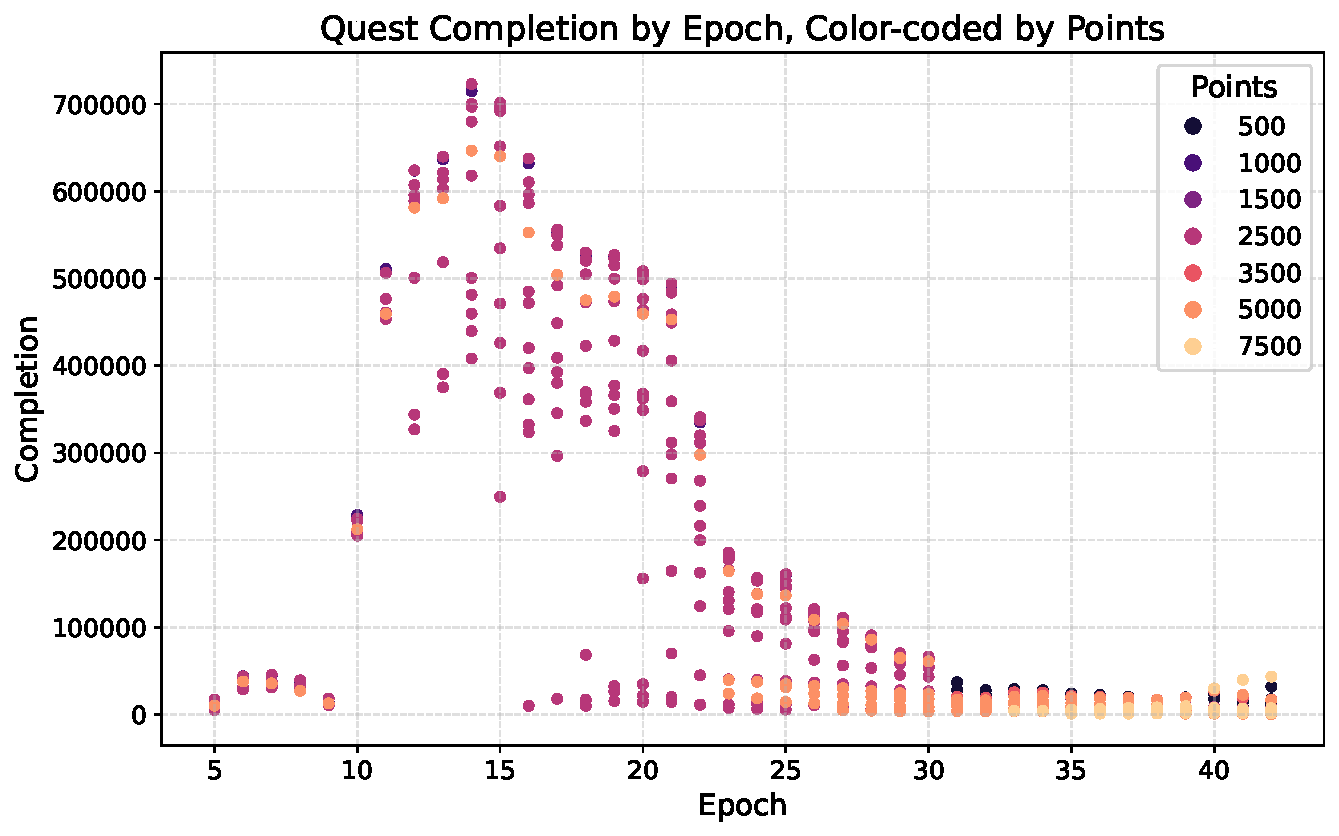
\includegraphics[width=0.8\textwidth]{figures/points.pdf}
    \caption{Reward amount (in non-monetary points) of different quests offered from Epoch 5--42. Completion rates do not correlate with points, indicating other contributing factors.\label{fig:points}}
\end{figure}

Points have long been a key element in gamification systems, primarily used to incentivize specific behaviours or actions, such as educational tasks, objectives in a game, or fostering loyalty through purchases at a business. For quests, points are usually presented in leaderboards---a public, ordered ranking of users and their points, which can boost competition, and result in users striving not merely to collect points but to climb the ranks. Leaderboards have a downside too. Newcomers might feel deterred by the seemingly insurmountable gap between themselves and top-ranked users, and excessive focus on ranking can foster cheating or the transacting of user profiles (with their points).

To what extent do points motivate users? Consider Figure~\ref{fig:points} where it shows a dot for each quest offered in each epoch (x-axis) and the number of times it was completed (y-axis). The shape of the curve follows the overall trend (Figure~\ref{fig:events}). The dots in Figure~\ref{fig:points} are colour-coded for how many points the user receives for completing the quest. A simple hypothesis is that quest completions would correlate positively with the number of points. Using the Spearman correlation, we found that correlations across epochs ranged from -0.115 to -0.870, with no epoch showing a significant positive monotonic relationship. In other words, the rank ordering of points and completions does not reveal any consistent patterns—for instance, higher points do not reliably correspond to more completions.

Finally, we note that in the later epochs, a strong negative monotonic relationship emerged, indicating that higher-point quests were completed less frequently. This was an intentional design decision, as more challenging quests were assigned higher point rewards to incentivize completion. As the data suggests, higher point rewards alone were not associated with increased engagement for these harder quests. Instead, quest difficulty, and other factors that act as deterrents, are more strongly associated with variations in task completion. This finding highlights the need to consider additional factors (RQ2–RQ5) to better understand the predictors of task completion.

% = = = = = = = = = = = = = = = = = = = = = = = = = = = = = = = = = = = = = = = = = =

\subsection{RQ2: Task Difficulty}

\begin{figure}[t]
    \centering
    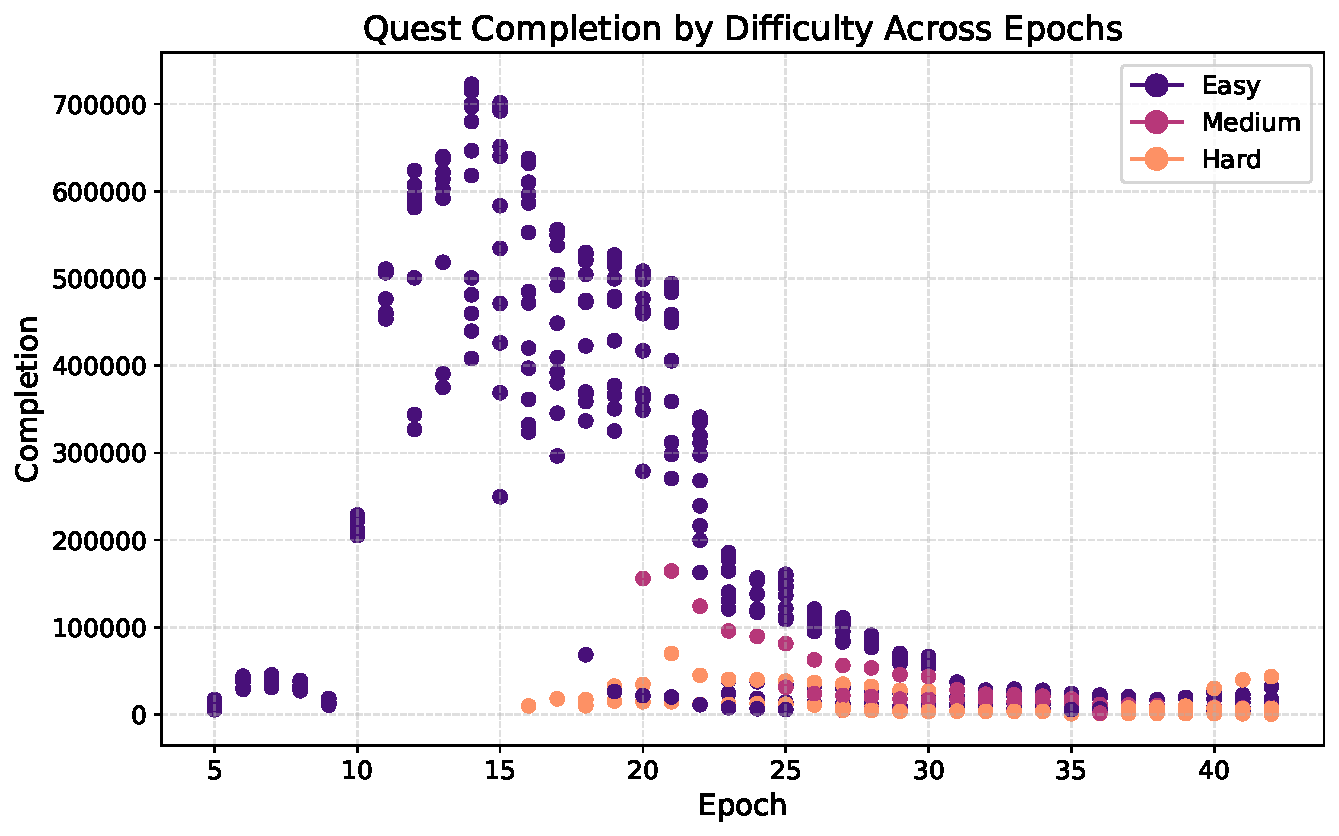
\includegraphics[width=0.8\textwidth]{figures/difficulty.pdf}
    \caption{Quest difficulty is strongly associated with completion rates, with easy quests (purple) completed most often and difficult quests (orange) completed least often. Variance in the right tail (epochs 40+) correspond to offering medium quests (pink) with tokens of monetary value (see RQ5).\label{fig:difficulty}}
\end{figure}

The first research question addresses points, which pull users toward certain quests. On the other side, frictions or deterrents may push users away from certain quests. RQ2--4 address three of these: difficulty, cost, and minimum token requirements (or thresholds). In RQ2, we consider task difficulty. We classify all quests based on (i) completion time, as measured by lead researcher who completed each quest modelling average user behaviour; and (ii) external dependencies that are out of the user's direct control, such as waiting for a response from another system, interacting with other users, or relying on network availability:

\begin{itemize}
\item Easy: quest takes less than 1 minute and has no external dependencies.
\item Medium: quest takes 1--2 minutes and/or has external dependencies but dependencies require minimal effort to resolve.
\item Hard: quest takes longer than 2 minutes and/or has significant external dependencies.
\end{itemize}

An example of an easily resolved external dependency would be finding another player for a game where many players are available at all times. By contrast, if players were rarely available, the quest would be ranked hard instead of medium. If a quest falls between two levels, we will typically classify it as the easier of the two. 

As evident from Figure~\ref{fig:difficulty}, difficulty is strongly associated with task completion. Using Spearman correlation (with reversed difficulty mapping), we found that correlations across epochs ranged from 0.121 to 0.663, mostly indicating a positive monotonic relationship. Easier tasks consistently had higher completion rates. 

Nevertheless, in certain epochs, the positive correlation was not as strong. As shown in Figure~\ref{fig:difficulty}, some medium or hard quests were completed more frequently than easier tasks, suggesting that other deterrents or negative incentives may be more strongly associated with quest completion than difficulty alone. This observation is further explored by analyzing factors such as cost and thresholds in subsequent sections.

% = = = = = = = = = = = = = = = = = = = = = = = = = = = = = = = = = = = = = = = = = =

\subsection{RQ3: Cost}

\begin{figure}[t]
    \centering
    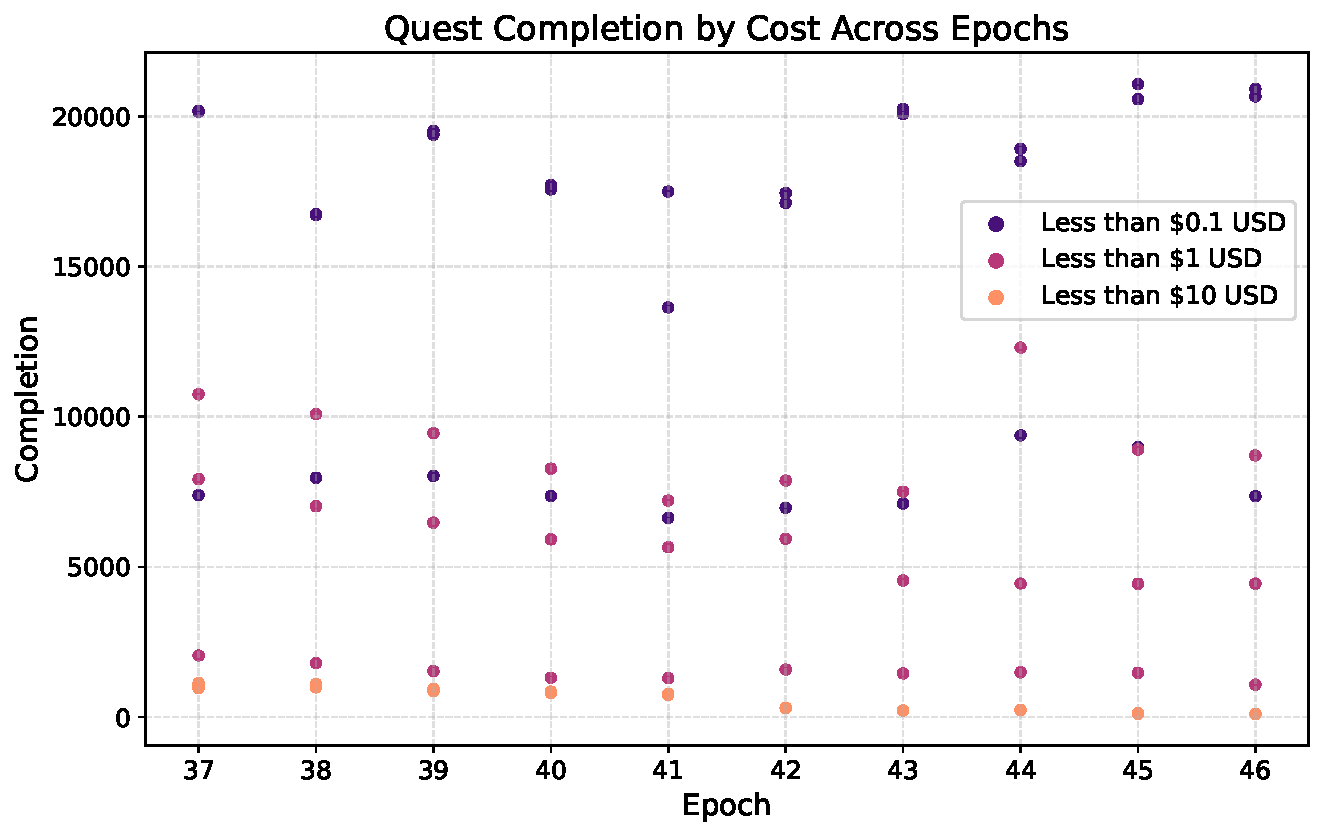
\includegraphics[width=0.8\textwidth]{figures/cost.pdf}
    \caption{Quest cost is strongly associated with completion rates, with cheaper quests (purple) completed most often and more expensive quests (orange) completed least often.\label{fig:cost}}
\end{figure}

All quests involving an on-chain transaction will have non-zero cost to complete, as the user needs to pay the transaction fee. The more complex the task, the larger the gas fee could be. For example, if a quest involves using a DeFi service, the service itself may charge fees on top of the gas costs. Quests that involve bridging assets between (layer 1) Ethereum and the blockchain project seemed particularly disliked, likely due to gas fees being high on Ethereum. 

In Figure~\ref{fig:cost}, we show a selection of quests from epochs 37--46 (later quests demonstrated more variety in complexity) and coded their cost into three colours: purple is less than \$0.10 USD, pink is less than \$1.00 USD (and more than purple), and orange is \$1.00 USD and more (no quest was greater than \$10 USD but some cost greater than \$5.00 USD). Quest costs in USD were computed using token exchange rates at the time of each transaction, based on price data provided by CoinGecko, aligning precisely with the prices displayed to users on the quest platform UI. The analysis of quest completion data revealed a clear trend: quests with a cost under \$0.10 USD are consistently completed by a larger number of users across all epochs, while those costing between \$1 and \$10 USD see minimal engagement. This pattern suggests that cost is strongly associated with lower engagement in high-cost quests. Given this observed relationship, quest designers may benefit from considering alternative incentives or cost structures.

Using the Spearman correlation, we found that correlations across epochs ranged from -0.843 to -0.896, consistently showing the strongest monotonic relationship among all research questions.
As shown in Figure 3, the rank ordering of cost and completions reveals a clear pattern—less costly quests (e.g., purple, costing less than \$0.10) are completed far more frequently than higher-cost quests (e.g., orange, costing up to \$10). This finding reinforces the idea that cost is strongly associated with lower task completion.

Since cost showed the strongest correlation, we infer that users are not completing quests randomly, nor are they primarily motivated by mastery or loyalty. Instead, their behavior suggests a tendency to minimize cost, aligning with patterns commonly associated with Sybils or automated bots. This observation led us to the next research question, where thresholds were introduced to user wallets to investigate their impact on completion rates and assess whether financial deterrents influence engagement in a more structured manner. 


% = = = = = = = = = = = = = = = = = = = = = = = = = = = = = = = = = = = = = = = = = =

\subsection{RQ4: Thresholds}

\begin{figure}[t]
    \centering
    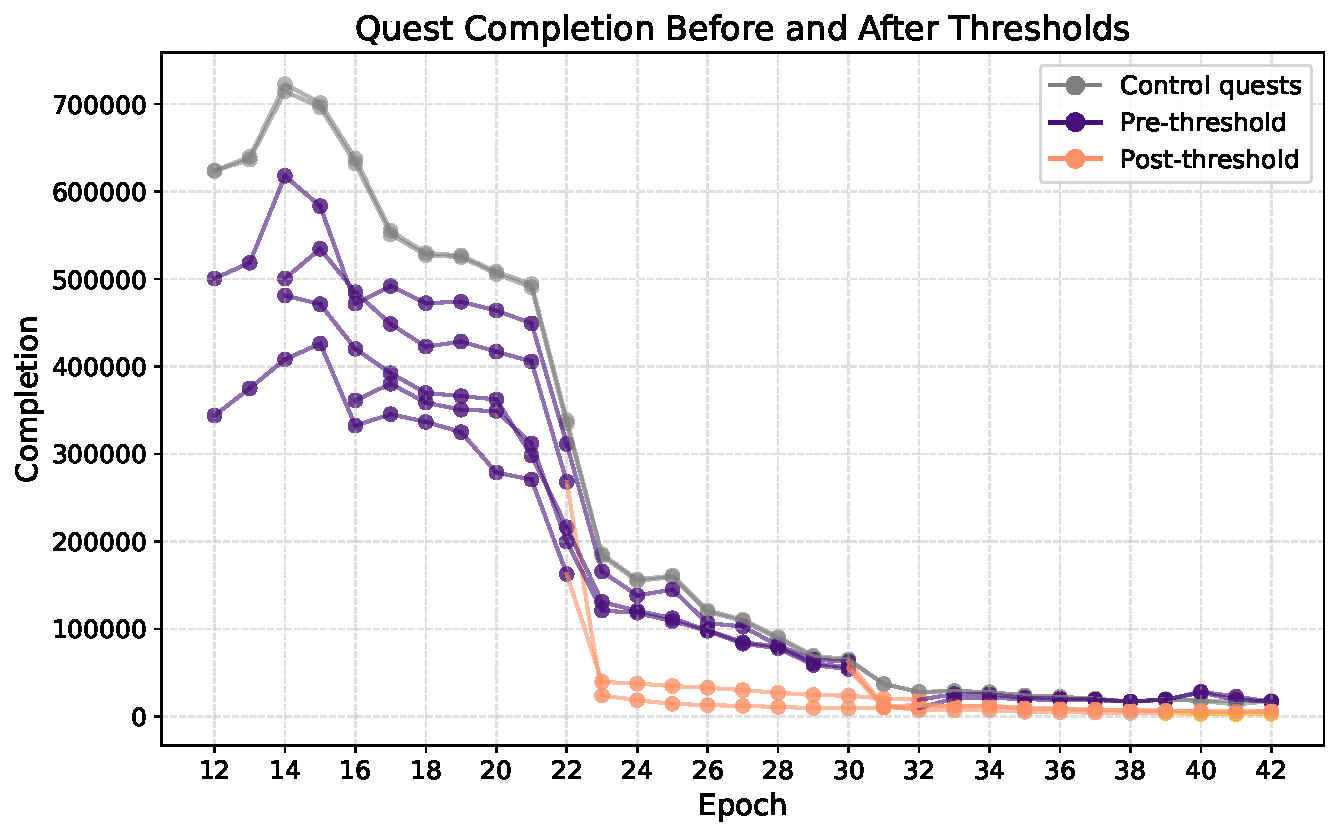
\includegraphics[width=0.8\textwidth]{figures/threshold.pdf}
    \caption{The implementation of a minimum threshold of tokens for quest completion is associated with an immediate decline in completions for quests that previously ran without thresholds (orange segment compared to the purple segment). The grey lines represent highly completed tasks as a control group.\label{fig:threshold}}
\end{figure}

We consider one last complication for users: quests that can only be completed by accounts with a minimum threshold of tokens. Thresholds are used to combat farming and bots, which we discussed further in the next section. For now, we simply measure their correlation with quest completion. 

Consider Figure~\ref{fig:threshold}. It shows 5 quests (purple lines) that ran for multiple epochs without a threshold, and then a threshold was applied to them (purple lines turn orange). In a few cases, the threshold was removed and the line goes back to purple. As a control group of quests for comparison, the grey line shows 5 highly completed quests (all simple token transfers). Throughout all epochs, these tasks had no threshold requirements for completion, and no thresholds were added at any point during the measurement. Most thresholds were in the native token on the blockchain project, and the amount of tokens required were worth between \$1 and \$10 USD. Some thresholds were in small amounts of ETH (0.002) or BTC (0.000125). 

As apparent from the figure, the implementation of a threshold is associated with an immediate decline in quest completion. The purple lines follow the same trend as the grey (control) lines (dampened by not being easy tasks) until the threshold is implemented, and then plummet. One might hypothesize that bots and farmers would take a few epochs to update their scripts or acquire threshold tokens, but the association appears sticky with no future uptick. When the threshold is removed, the quests' completion rates return to levels similar to those observed in the control group.

For example, one quest was completed 268,104 times in epoch 22, just before a threshold of approximately \$10 USD was introduced at epoch 23. Following the enforcement of the threshold, completions dropped dramatically to 23,923— a 91\% decrease. When the threshold was removed at epoch 33, the quest saw a significant rebound, with completions more than doubling, increasing by 112.8\%.

Similarly, another quest, which had a threshold of approximately \$5 USD enforced at epoch 23, experienced a 75.8\% drop in completions. After the threshold was removed at epoch 33, completions increased by 33.4\%. 

These examples highlight a substantial association between thresholds and lower user participation, as well as an association between the removal of thresholds and a return to higher completion rates.


% = = = = = = = = = = = = = = = = = = = = = = = = = = = = = = = = = = = = = = = = = =

\subsection{RQ5: Rewards with Monetary Value}

\begin{figure}[t]
    \centering
    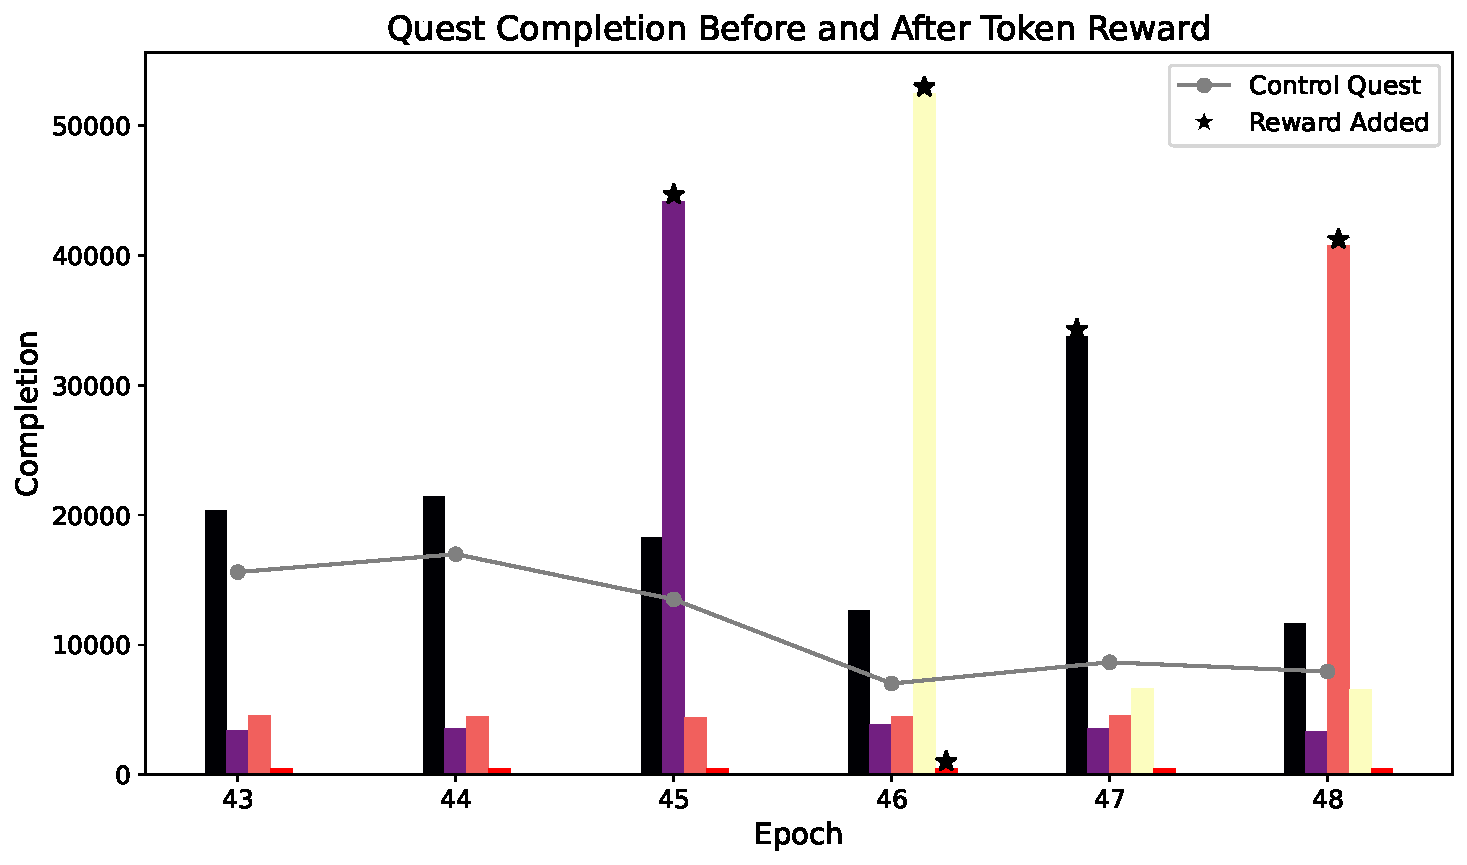
\includegraphics[width=0.8\textwidth]{figures/tokens.pdf}
    \caption{Five quests (by colour) that were offered over multiple epochs with a reward in non-monetary points (bars with no star) and also offered for one epoch with a token reward (bar with star). The grey line shows an average of task completion for the other quests over the same epochs. The chart shows that offering tokens (with a monetary value) as rewards is associated with higher quest completion. \label{fig:tokens}}
\end{figure}

Consider Figure~\ref{fig:tokens} which depicts 5 quests by colour, each offered over epochs 43--49 (expect the yellow quest, which was first offered in epoch 46). For most epochs, the completion award was non-monetary (loyalty or experience) points, as we have analyzed in the previous section. In contrast, for one epoch (shown with a star), alongside the usual point rewards, specific quests were selected for a token reward (in the native token of the blockchain project) which had a small monetary value of ~\$0.10 USD. The grey line shows the completion rate of the control quest offered across the same epochs.

This was not a perfect experiment for assessing the association of monetary rewards with quest completion, as the rewards were capped at \$5000 USD, allowing a maximum of 50,000 users to claim rewards before they ran out. Further, if two quests offered monetary rewards in the same epoch, they would compete against each other until the tokens were depleted (see epoch 46 in Figure~\ref{fig:tokens}).

Despite these defects in the data, the results are insightful: even with a minimal reward, completion rates surged. The highest increase was over 12x for a quest typically completed by around 3,500 users. With the token reward, this quest (purple in Figure~\ref{fig:tokens}) saw 44,196 completions. Directly after the token reward for this quest was removed, the completion rate dropped back to its original levels before the reward was introduced. 

These data reveal that the introduction of a token reward is associated with a spike in completions, while the removal of the reward corresponds with a decline back to earlier levels. These spikes suggest that token rewards do not foster loyalty or habitual engagement but rather create a purely transactional relationship. Users appear to compare the cost to the reward and only engage when there is a clear opportunity for profit.

In epoch 46, two quests with token rewards showed different outcomes. While the yellow quest, which had a low cost, saw a significant increase in completions, the red quest, which had a cost higher than the reward, experienced no increase at all. If users were engaging with the platform out of loyalty or mastery, they would have completed the red quest as well as the yellow quest. However, this did not happen: users who claimed the reward for the yellow quest did not complete the red quest, leaving the reward for the red quest unclaimed.

% = = = = = = = = = = = = = = = = = = = = = = = = = = = = = = = = = = = = = = = = = =

\subsection{RQ6: Bots and farming}

We currently lack data revealing how many task completions come from unique individuals versus repeat participants using multiple addresses (farming), whether by manual sybils or automated bots. Both human users and bots seem drawn to quests with higher monetary rewards, simpler tasks, and lower costs, making it difficult to distinguish them based on these factors alone.

\paragraph{Possible distinguishers.} The Fogg Behavior Model~\cite{Fogg09} was proposed to understand how well commercial products integrate into users’ daily routines, and we see it as relevant to the design of quests. The model is expressed as the pseudo-equation $B=MAP$ where a behaviour (B) requires simultaneous motivation (M), ability (A), and a prompt (P) (formerly known as a trigger). If any one of these components is missing or inadequate, establishing a specific behaviour is challenging or impossible.

Under this model, do non-transactional users (`genuine users') and farmers, bots, and scripts (`bots') exhibit the same behaviour (B) when the inputs (MAP) are the same? The answer seems to be no. Both are motivated (M) when the benefits outweigh the costs, but genuine users are largely unaffected when the benefits are small (\cf picking up a penny off the road). By contrasts, bot farms will immediately engage because they can use scale to accumulate a tiny profit from each quest into a material amount (\cf picking up thousands of pennies).

Bots are more responsive to prompts (P) (\eg a new quest is available) because they are scripted to listen for them, whereas genuine users need rely on marketing, reading push notifications, or remembering to check the website. At an extreme, bots monitoring the blockchain's mempool for profitable transactions might discover profitable quest completions without knowing anything about the quests themselves. Such bots are called general-purpose Maximal Extractable Value (MEV) bots~\cite{DGK+20} and they simply re-stage every transaction they see before the transaction is confirmed, and if they determine it will be profitable for them to originate, they will front-run the original transaction. The ability (A) to react quickly to prompts, and at the extreme, front-run other transactions, is another distinguishing feature of bots versus genuine users. 

Finally, we observe that to complete a quest, an address needs to hold an adequate amount of currency and/or number of tokens to have the ability (A) to pay gas fees and any other fees associate with the quest. Genuine users are likely to hold more than the minimum amount and to have held it for some period of time. By contrast, farming operations have to divy the tokens across many addresses, meaning there is likely a correlation between these addresses being newly created and holding a minimal amount of capital.

Putting this together, we suggest three heuristics that may help distinguish genuine users from bots. There are likely exceptions to all of them (\eg genuine humans running scripts) but we hypothesize that they would do better than random guessing at determining if a given address is a genuine user or a bot.

\begin{itemize}
\item Heuristic 1: If a quest goes from gradually becomes profitable over time, bots will be sensitive to the exact moment it becomes marginally profitable and act.\item Heuristic 2: If a quest requires a threshold (minimal amount of tokens), bots will be sensitive to ensuring the address meets but does not exceed the threshold amount. 
\item Heuristic 3: If a (profitable) quest is announced (especially unexpectedly), bots will be the quickest to react.
\end{itemize}

Finally we emphasize that if these heuristics were deployed in a way that harmed bots (\eg banning rather than passive measurement), bots can adjust their behaviour to evade detection, resulting in a `cat and mouse' game between farmers and quest creators. 

\paragraph{Quest design ideas.} In the absence of concrete measurements and based on these insights, we outline several ideas for collecting more robust data, and designing better quests that can help identify and quantify farming activity.

Building on heuristic 1, if costs (\ie gas fees, service fees, buying a token or NFT as part of the quest, \etc) are slightly higher than rewards (\ie tokens of monetary value received for quest completion), genuine users might be happy they are at least receiving a subsidy for a quest they would complete anyways, while bots will avoid unprofitable tasks. When benefits are slightly higher than costs, bots will engage. For many quest designs, the profitability of the quest could be due to external factors such as fluctuations in gas rates or in the value of the token received. This could create the conditions for a `natural experiment' where a quest is offered over an epoch, but its profitability fluctuates between negative and positive. Activity spikes when it becomes positive could be largely attributed to bots.

A second idea corresponds to heuristic 2 and the use of thresholds (RQ5). If a quest can only be completed by addresses holding at least $X$ tokens, bot farms may need to move $X$ tokens between their addresses. In general, clustering algorithms can use heuristics on blockchain data to suggest addresses belonging to the same user, and inducing these kinds of transfers could help make the pattern more distinguishable. Farming can also be frustrated by requiring each address to have held $X$ tokens for a certain period of time (days or weeks). Of course, if a farm with $n$ bots holds more than $n\cdot X$ tokens, farms will be unaffected by the use of thresholds. 

A final idea builds on heuristic 3. In the quest system we studied, a smart contract was randomly replenished with a fixed daily reward pool of \$500. Pre-enrolled participants with sufficient loyalty points could claim a nominal reward (\$0.01 or \$0.025, depending on tier) until the pool was depleted. 

% !TEX root = ../main.tex

\begin{table}[t]
    \centering


    \begin{tabular}{c | c | m{3.5cm} | m{3.5cm}}
    \hline
    \textbf{Day} & \textbf{Refill Time} & \textbf{Immediate Claims (within 2 minutes)} & \textbf{Duration to Deplete Rewards } \\
    \hline
    1  & 13:00:00 & --   & 12h    \\
    2  & 12:02:17 & 200  & 1h50m  \\
    3  & 13:25:45 & 500  & 1h33m  \\
    4  & 12:09:01 & 1500 & 58m    \\
    5  & 12:45:58 & 350  & 1h30m  \\
    6  & 12:27:53 & 200  & 1h40m  \\
    7  & 13:30:17 & 1500 & 28m    \\
    8  & 16:30:07 & 300  & 2h41m  \\
    9  & 11:59:57 & 1500 & 27m    \\
    10 & 11:59:57 & $>1500$ & $<30$m \\
    11 & 11:59:57 & $>1500$ & $<30$m \\
    \hline
    \end{tabular}
        \caption{Daily Refill Times and Depletion Data.\label{tab:claims}}
    \end{table}
    

Looking at Table~\ref{tab:claims}, we observe a marked decrease in the time taken to deplete all rewards as the days progressed. This would be expected if participants developed a habit of claiming rewards at a consistent daily time; however, column 2 indicates that refill times varied significantly, making it difficult for users to predict when rewards would be replenished. The key observation lies in the number of claims recorded within the first 2 minutes of refilling the contract, demonstrating the dominance of automated systems.

On Day 7, for instance, despite a one-hour delay in the refill time, approximately 1,500 claims were made within 2 minutes. The following day, a more drastic delay of 3 hours saw claims drop to 300, likely due to the implementation of rate-limiting and a mandatory wait period between claims. Notably, this led to a temporary spike in the time required to deplete all rewards, which rose to 2h41m. By Day 9, however, the refill occurred 4.5 hours earlier, and bots had clearly adapted, with 1,500 claims occurring within 2 minutes and the time to deplete rewards dropping to 27 minutes. Finally, following the introduction of an automated daily refill schedule on Days 10 and 11, the system reached its operational minimum, with rewards being depleted in under 30 minutes and claims stabilizing at ~1,500 within the first 2 minutes.

Although these observations are suggestive, they are not conclusive for two reasons: (1) a backend system (using Cloudflare) attempted to block or rate-limit repeated bot requests, requiring multiple submissions for a single on-chain claim to succeed, and (2) the smart contract batched multiple claims into a single transaction, potentially delaying some submissions that had occurred earlier. A more direct on-chain approach—where each wallet claim corresponds to an individual transaction—would likely yield clearer data.

By studying claims made very quickly or even launching a quest such as `make a claim within the first 2 minutes after rewards were added,' it is likely that observed completions could be attributed to bots. Even without conducting in-depth analysis, many teams (based on personal conservations and social media) sense that their platform has attracted a significant number of bots. In some instances, these teams recognize that their applications or quest systems have effectively become `farming machines' for bots. However, as discussed in the next section, awareness of such bot activity does not necessarily compel teams to intervene; in certain scenarios, they may even be incentivized to sustain it.

% = = = = = = = = = = = = = = = = = = = = = = = = = = = = = = = = = = = = = = = = = =

\section{Stakeholder Analysis} 

% !TEX root = ../main.tex

\renewcommand{\arraystretch}{1.3}

\newcommand{\yay}{\textcolor{black}{$\Uparrow$}\xspace}
\newcommand{\nay}{\textcolor{red}{$\Downarrow$}\xspace}
\newcommand{\neu}{}
\newcommand{\con}{\textcolor{blue}{$\circlearrowleft$}\xspace}

\begin{table}[t!]

\adjustbox{}{

\begin{tabular}{p{5cm}m{0.5cm} m{0.5cm} m{0.5cm} m{0.5cm} m{0.5cm} m{0.5cm} m{0.5cm} m{0.5cm}}

\multicolumn{1}{l}{~} &
\headrow{Enhances activity} & 
\headrow{Enhances education} & 
\headrow{Enhances lock-in}  & 
\headrow{Resilient to farming} & 
\headrow{Revenue for project} & 
\headrow{Revenue for third parties} & 
\headrow{Revenue for user} \\ \hline 

\multicolumn{1}{c}{\textbf{Stakeholder}} & \multicolumn{7}{c}{\textbf{Deliverables}} \\

\hline
 						% txs	%edu	%lock	%farm	%plat	%tps	%user
Project: Developers			& \yay	& \yay	& \yay	& \con	& \yay	& \neu	& \neu 	\\ \hline
Project: Executives			& \yay	& \yay	& \yay	& \nay	& \yay	& \yay	& \con 	\\ \hline
Project: Investors			& \yay	& \yay	& \yay	& \con	& \yay	& \neu	& \yay 	\\ \hline
Project: Token Holders		& \yay	& \neu	& \yay	& \nay	& \yay	& \neu	& \neu 	\\ \hline

Users: Transactional			& \neu	& \neu	& \neu	& \neu	& \neu	& \neu	& \yay 	\\ \hline
Users: Exploratory			& \neu	& \yay	& \neu	& \neu	& \neu	& \neu	& \neu 	\\ \hline
Users: Loyal                             & \yay	& \yay	& \yay	& \yay	& \neu	& \neu	& \neu 	\\ \hline

Third Party: DApps			& \yay	& \yay	& \yay	& \yay	& \neu	& \yay	& \neu 	\\ \hline
Third Party: Quest Platforms	& \yay	& \neu	& \nay	& \neu	& \neu	& \neu	& \yay 	\\ \hline
Third Party: Metric Platforms	& \neu	& \neu	& \neu	& \yay	& \neu	& \neu	& \neu 	\\ \hline

\end{tabular}
} % end resizebox

\caption{A set of stakeholder groups and potential deliverables from a quest platform. Each cell indicates the priority of the stakeholder for the deliverable: empty means the priority is ambivalent to moderately favourable, \yay means it is high priority, \nay means the stakeholder opposes the deliverable, and \con indicates conflicting priorities within the stakeholder group. \label{tab:stake}}
\end{table}

\renewcommand{\arraystretch}{1.0}



A deeper question is what stakeholders actually prioritize. Is it the elimination of bots, metric boosts, revenue, other things? We conduct a \textit{stakeholder analysis} (first used by Clark \etal for secure email systems~\cite{CvORSZ21}). Table~\ref{tab:stake} provides, as rows, a set of stakeholder groups and, as columns, a set of possible deliverables a quest system might provide. Deliverables are phrased to be generally favourable, so most stakeholder groups will default to being moderately in favour or, at worst, ambivalent (empty cell). Cells showcase when there is strong support, strong opposition, or internal conflict over a priority. This table helps us locate tensions between stakeholder groups.

The first column describes the main function of a quest system: to enhance genuine user activity, a goal no stakeholder group opposes. Quest completions are not `genuine' in the sense of economic activity---quests are completed for the sake of the quest, which is superficial. However we use `genuine' to distinguish from attempts to game the quest system (which we will turn to in column 4). In the second column, again no stakeholder group opposes quests with educational value for users, while such quests are strongly preferred by exploratory users.

As of writing, the blockchain space is fragmented with many competing L1s, L2s, and services for common on-chain tasks (\eg DEXes, lending protocols, leveraged trading, \etc). Market share and user retention is a basic business goal of projects and their loyal users. Projects offering quests will typically only include quests that use the project, while quest platforms (the `loyalty layer') offer a single hub for quests across multiple projects. Their niche is based on quests being spread across competitors. Occasionally projects will join quest platforms and then poach users for their own internal quest systems---called a `vampire attack.'

The most contentious deliverable is the elimination of farming---bots, sybils, and other methods used by transactional users to automate task completion. The basic tension is that inflated completion metrics (\eg monthly active users (MAU)) paint the picture of a fast-growing, robust user base, but its illusionary nature (`vanity metrics') could compromise credibility or collapse if transactional users exhaust the opportunities and move on to newer projects. Anti-farming measures are supported by DApps chosing a project to deploy on, favouring platforms with large genuine user bases. Joining them are metric platforms, which provide rankings of most popular projects, will lose credibility and relevance if it is easy for projects to use quests to game their metrics and climb the leaderboard. Loyal users receive more recognition when their contributions are not drowned out by a sea of fake engagement.

We expect project-based stakeholders to tacitly support farming (or at least turn a blind eye). Investors understand this when they are in a position of selling or exiting, however they want a real picture of the user base when buying into a project---thus are in internal conflict. Developer teams are similar, wanting ground truth when choosing between projects to work on and wanting success once in a team. 

When it comes to the final three columns, which emphasize the main groups that might make revenue from quests, there are no big surprises. No one opposes stakeholder capturing some revenue and stakeholder groups are self-interested, prioritizing revenue to themselves. In our evaluation, we assume revenues are non-zero sum---that is, revenue to one stakeholder group does not siphon profit from the others.

% = = = = = = = = = = = = = = = = = = = = = = = = = = = = = = = = = = = = = = = = = =

\section{Concluding Remarks}

It is easy to see why quest systems are popular. In Web3, reaching users with a new project is challenging. Web3 does not operate with an ``app store'' that is easy to browse. Beyond bringing in new users, quests promise to educate users and build loyalty. However if quests are too successful, farming and bots may follow real users. Farming is a kind of ``Midas touch'' for projects, immediately boosting metrics and engagement. But ultimately, it forces teams into an uncomfortable dilemma: either admit that much of their previous participation came from bots—risking tension with partners, genuine users, and investors—or remain silent and appear to lose the bulk of their user base. Relying on bots to attract additional users or applications is a perilous strategy, particularly for teams that lack a clear, long-term plan to manage bot activity and know when to stop engaging with them.





